\chapter{Technical Foundations and Candidate Models}
\label{ch:foundations}

\section{Common Mathematical Notation and Prediction Formulation}
Let $i$ index a prediction unit, $g(i)$ its dependence group, and $m\in\{v,s\}$ the visual and sensor inputs. The available observations are $x_i^{(m)}$, an availability indicator $a_i^{(m)}\in\{0,1\}$, and optional process or measured-quality context $u_i$. The target $y_i$ is continuous in regression and binary in failure classification, where $y_i=1$ denotes failure. An encoder $f_m$ yields an embedding $h_i^{(m)}$; a prediction head yields a scalar score $z_i^{(m)}$ and, after an explicitly specified calibration map, a probability $p_i^{(m)}$.

The fusion stage can receive an embedding, a score, or a probability. A probabilistic classifier estimates the chance of the target outcome. A fitted calibration map adjusts that estimate against observed outcomes in training data. A logit $\ell(p)=\log[p/(1-p)]$ requires clipping at the probability boundaries in numerical code. Each case study specifies which inputs its fusion model receives and how those inputs enter the model.

\section{Visual Representations}
\subsection{Convolutional Feature Extraction and Spatial Pooling}
A convolutional encoder maps a frame $I_t$ to feature maps $F_{t,k}\in\R^{C_k\times H_k\times W_k}$ at scale $k$. Global average pooling forms $r_{t,k,c}=(H_kW_k)^{-1}\sum_{h,w}F_{t,k,c,h,w}$. Concatenating scales gives $r_t=[r_{t,1};\ldots;r_{t,K}]$. A mean over selected frames then gives $\bar r=T^{-1}\sum_t r_t$. This is a compact descriptor of a complete observation window. Spatial pooling discards explicit object position and local correspondence; temporal averaging discards frame order. The resulting model can exploit changes in visual content but does not implement learned temporal attention.

A strong convolutional reference remains necessary when Transformer components motivate an architecture search. ViT's advantage depends on pretraining scale, with smaller-data comparisons favoring convolutional inductive biases \citep{P010}. Video Swin adds local spatiotemporal attention and shifted windows, while its evaluation cost depends on temporal clips and spatial crops \citep{P013}. These papers establish candidate mechanisms, rather than superiority to the frozen CNN under the industrial sample support and budgets evaluated here.

\subsection{RT-DETR Architecture and Component Roles}
RT-DETR is a real-time detection architecture with a convolutional backbone, a hybrid encoder for multiscale feature interaction, and a query-based decoder that predicts detections \citep{Zhao2024RTDETR}. These blocks have different purposes. Backbone maps encode local and hierarchical image patterns. The hybrid encoder combines within- and across-scale information. The decoder and prediction heads produce object-level outputs. A checkpoint trained for detection may supply weights to any chosen subset of these blocks, but the checkpoint's origin does not establish which blocks a downstream program executes.

\subsection{Backbone Extraction Versus Hybrid-Encoder or Full-Detector Execution}
The core REASSEMBLE visual extractor uses the ResNet18-vd CNN backbone inside the pretrained RT-DETR-R18vd checkpoint (\texttt{PekingU/rtdetr\_r18vd}). After loading the detector, the implementation selects its backbone and freezes its weights. It spatially averages three feature maps to form an 896-dimensional descriptor per frame, then averages the descriptors of 16 frames. A separately trained binary head predicts the action outcome. This forward path bypasses the hybrid Transformer encoder, detection decoder, and box heads.\ev{Executed core visual path}{\EvidenceRef{E064}{load\_visual, extract}, \EvidenceRef{E065}{VisualHead}}

PHM's scalar-regression route is different. It invokes the Ultralytics prediction path with a frozen RT-DETR-L model and hooks three multiscale maps. Pooling produces 768 features; the saved extraction adds latency, making the head input 769-dimensional. The PHM head therefore receives both image content and a timing covariate. REASSEMBLE calls only the detector's CNN backbone for the core comparison. Later CNN-versus-spatial-encoder studies are additional recipes with their own feature widths and budgets.\ev{PHM component map}{\EvidenceRef{E033}{extract\_features, train\_head}}

\subsection{Frame Sampling, Feature Aggregation, and Temporal Modelling}
Fixed sampling selects a reproducible number of frames across a complete action or episode. It makes sequence cost predictable and prevents longer clips automatically producing more visual tokens, but can miss brief contact or failure events. A frame mean is invariant to permutation. Boundary pooling or temporal bins retain some coarse position; a GRU or temporal Transformer learns order-dependent interactions. These alternatives address different hypotheses and must be evaluated using matched sampling and fitting rules before a difference can be attributed to temporal modelling.

The core REASSEMBLE route uses 16 deterministic hand-camera frames resized to $640\times640$, divided by 255, without additional ImageNet mean/standard-deviation normalization. These are actual recipe choices rather than generic defaults for every RT-DETR implementation. Dataset examples in Chapter~6 show sampled observations; they are illustrative, not independent evidence of label correctness or a performance effect.

\subsection{Frozen Extraction and Visual Fine-Tuning}
Frozen extraction keeps encoder parameters fixed while fitting a head. Fine-tuning changes some or all encoder parameters. A comparison also depends on normalization-layer state, augmentation, learning rates, early stopping, batch size, and optimization steps. A fixed embedding cache can make nested evaluation practical; an end-to-end model may require a new backbone fit inside every inner split. The additional computational burden is not a reason to treat an unmatched budget comparison as an isolated test of freezing.

Generic COCO initialization, REASSEMBLE donor initialization, and target-domain head fitting are distinct interventions. A cached donor embedding proves that extraction occurred; it does not prove that a downstream classifier and fusion comparison completed. In ViFailback, donor feature extraction preceded the completed downstream fits. Chapter~8 compares those fits with the matched target-task control.

\section{Sensor and Time-Series Representations}
\subsection{Statistical and Signal-Derived Features}
For a channel sequence $x_1,\ldots,x_n$, common summaries include mean, standard deviation, extrema, quantiles, root-mean-square amplitude, and changes across the window. For example, $\mathrm{RMS}(x)=\sqrt{n^{-1}\sum_t x_t^2}$. These features trade temporal detail for compactness and can provide a strong reference when sample support is limited. Spectral features additionally summarize frequency content, but their interpretation depends on the physical sampling rate and the preprocessing window. A time series resampled to action progress is not interchangeable with a raw uniformly sampled vibration waveform.

REASSEMBLE's statistical branch uses ten statistics for each of 22 channels, producing 220 features. Its channels combine force, torque, gripper, joint effort, and joint velocity measurements. MSM uses its specified controller-measurement adapter. PHM uses engineered minute-level sensor/context features in the retained regression path. The model name alone cannot make these three input definitions equivalent.

\subsection{PatchTST Architecture}
PatchTST represents a time series as patches rather than treating each timestamp as a separate token. Its original formulation combines patching with channel-independent processing, enabling a Transformer to model temporal structure within channels \citep{Nie2023PatchTST}. An architecture inspired by this design can be initialized from scratch; that is not pretrained time-series weight transfer. The thesis uses the term PatchTST with the implementation specified, because PHM's custom regressor and REASSEMBLE's Hugging Face classifier differ in patching, aggregation, targets, and fitting.

\subsection{Patching, Sequence Length, Padding, and Aggregation}
For sequence length $L$, patch width $P$, and stride $S$, an unpadded regular grid contains $1+\lfloor(L-P)/S\rfloor$ patches when $L\geq P$. Padding conventions can change that count. A patch embedding projects its values to a hidden vector, adds positional information, and passes the sequence through Transformer blocks. Pooling must specify whether all patches or only valid patches contribute.

REASSEMBLE resamples the action to 512 progress positions and 22 channels. Its scratch classifier uses width 32, two layers, four attention heads, feed-forward width 64, patch width 32, and stride 16, followed by patch averaging and channel concatenation before a 128-dimensional projection. Scaling is disabled inside the model because standardization is supplied externally. The implementation passes an observed-value mask to the model. The call alone does not establish that attention excludes every missing position.

PHM's custom default uses patch 16 and stride 8 with variable-length minute sequences. Its patch validity is based on any valid time within a patch, followed by masked aggregation. The source raises a batch-length-dependent grid concern; its numerical effect on historical scores remains unmeasured. PHM also predicts sorted profiles with positive increments, which remove tooth identity. That target representation cannot support a tooth-localization claim.\ev{Sensor implementation map}{\EvidenceRef{E031}{}, \EvidenceRef{E065}{SensorHead}}

Other learned time-series representations provide controls rather than interchangeable substitutes. TS2Vec uses a dilated CNN with hierarchical contrastive learning; substituting a Transformer in its backbone ablation lowers average classification accuracy \citep{P012}. MOMENT pretrains a masked-reconstruction Transformer across datasets, yet frozen-encoder classification still fits a supervised classifier and comparisons with specialized or shallow methods depend on task, metric and adaptation access \citep{P018}. Neither paper establishes a universal architecture ranking. Pretraining data, downstream labels and fitting budgets must accompany comparisons with the scratch-trained PatchTST branches.

\subsection{Representation Learning Versus Direct Prediction}
A learned encoder can be used to export an embedding, to predict the target directly, or to support a fusion head. These roles differ in where supervision enters. An encoder trained on all labels before a cross-validation split leaks target information even if a later classifier is refitted correctly. Conversely, a generic frozen encoder can be cached without using target labels, provided the cache remains tied to the correct sample identities and preprocessing. Checking for leakage in each fold requires identifying which samples were used to fit the preprocessing steps and which samples and labels were used to train the encoder and the final predictor.

\section{Prediction Models and Reference Baselines}
\subsection{Constant and Simple Reference Predictors}
A regression constant estimated from training data establishes whether a learned model improves on a basic location predictor under the selected loss. The training mean minimizes squared error, while the median minimizes absolute error in the training sample. For classification, a constant probability or a process-context model can expose target prevalence and contextual predictability. These controls are particularly important when a condition proxy is correlated with run order or when action identity predicts failure frequency.

\subsection{Linear and Logistic Models}
Ridge regression minimizes squared error plus an $L_2$ coefficient penalty. Logistic regression models $p(y=1\mid x)=\sigmoid(b+w^\top x)$ and typically minimizes penalized cross-entropy. Standardization, class weighting, regularization, and solver configuration are part of the recipe. The REASSEMBLE sensor reference searches $C\in\{0.1,1,10\}$ within training partitions. A fit of the same model family to two branch probabilities is a stacker, not a sensor representation. The fixed core F2 value $C=1$ is not described as a searched hyperparameter.

\subsection{Neural Classification and Regression Heads}
A compact head can use $h=\mathrm{ReLU}(W_1x+b_1)$, dropout during fitting, and a scalar output. In REASSEMBLE, the core visual and PatchTST heads used class-weighted binary cross-entropy. The original context gates used unweighted binary cross-entropy. Parameter counts describe the size of each fitted model. The visual head had 114,945 trainable parameters in addition to the frozen CNN. The sensor module had 109,505 trainable parameters across its PatchTST encoder, projection, and classifier, including 90,369 in the projection and classifier.

\subsection{Other Models Relevant to Retained Experiments}
Histogram gradient boosting (HGB) builds an additive tree model on binned features and captures nonlinear feature interactions without a sequence encoder. It is an important external sensor reference because outperforming a logistic sensor component does not establish superiority to a stronger sensor family. The ViFailback HGB comparison uses its actual validation-based candidate selection; MSM's HGB result belongs to its own controller-feature protocol. Appendix~C gives the configurations of the additional models.

\section{Fusion Mechanisms}
\subsection{Feature Concatenation}
Feature-level fusion applies a predictor to $[h_v;h_s]$, possibly after separate projection and normalization. If $q_m=\phi_m(h_m)$, one implementation is $p=\sigmoid(g([q_v;q_s]))$. It can learn cross-feature interactions while increasing fitted capacity. The retained PHM \texttt{fused\_all\_three} specifically concatenates embeddings from process-context, RMS and condition-indicator encoders before a scalar head. Despite the class name \texttt{LateFusionRegressor}, its forward path is feature fusion, rather than probability stacking or image--sensor inference. Equal final embedding width does not imply equal total encoder capacity.\ev{PHM feature-fusion inputs}{\EvidenceRef{E004}{section 12.4}}

\subsection{Uniform Prediction Averaging}
The core F1 baseline is $p_{\mathrm{F1}}=(p_v+p_s)/2$. It has no fitted combination parameters, although its branch predictors and calibrators are fitted. Its simplicity makes it a useful comparator for a learned stacker. Applying a sigmoid to the mean logit generally yields a different probability. When an input is missing, a rule for renormalization or abstention must be specified separately.

\subsection{Logistic Stacking}
The core F2 computation is
\begin{equation}
 p_{\mathrm{F2}}=\sigmoid(b+\alpha_v p_v+\alpha_s p_s).
 \label{eq:f2}
\end{equation}
The inputs are calibrated probabilities, not logits. Coefficients need not be positive or sum to one. F2 is therefore a fitted probability map with three parameters, rather than a convex weighted average. Its training inputs should exclude fitting the corresponding branch on that row's dependence group. In the retained core, branch out-of-fold construction excludes each scored row's recording, and outer assessment recordings are excluded from fitting. These exclusions do not establish independence of every later meta-validation stage: stacker validation reuses an outer-training prediction bank, creating the training-side dependency described in Chapter~6. This dependence occurs within the outer training set.

Model selection using evaluation data can bias its selected estimate \citep{P004}. This general risk does not itself establish outer-assessment leakage. That claim requires the actual preprocessing, fitting and prediction-bank dependencies \citep{P017}. Each of the three stages can use different training predictions for fitting the branch calibrator, the stacker and the decision threshold.

\subsection{Context-Conditioned Scalar Gating}
For context $u$, a gating network yields scores $q_m(u)$. Availability masks exclude missing branches before normalization:
\begin{equation}
 w_m(u,a)=\frac{a_m\exp(q_m(u))}{\sum_j a_j\exp(q_j(u))},\qquad
 p_G=\sigmoid\left(\sum_m w_m(u,a)\ell(p_m)\right).
 \label{eq:gate}
\end{equation}
The original gates use action context, quality context, or both. Their respective input widths are 6, 38, and 42 after including two availability indicators. The scalar logits are combined without a final intercept or post-gate calibration in the original formulation. This differs materially from F2's probability inputs and free intercept. A clean-score difference between them cannot be attributed solely to adaptive allocation.

Related gated mechanisms operate at different interfaces. Gated Multimodal Units mix hidden representations elementwise \citep{P006}, while attention bottlenecks exchange information through cross-modal tokens \citep{Nagrani2021MBT}. The executed gate above mixes two scalar logits. Adaptive fusion describes their family relationship; it does not make their computations equivalent or establish that the scalar gate learned cross-modal representations.

The gate operates on two scalar predictions. It is not token-level cross-attention between image regions and sensor patches. Inspecting its weights reveals allocation under the fitted model, but cannot establish the physical cause of failure or whether an operator would understand its decisions.

\subsection{Quality-Conditioned Interactions and Adaptive Extensions}
The anchored extension preserves a fitted F2 intercept and coefficients and learns bounded multiplicative adjustments:
\begin{equation}
 p_A=\sigmoid\left[b+\sum_m\alpha_m\{1+\tanh(h_m(u))\}p_m\right].
 \label{eq:anchored}
\end{equation}
Zero initialization of the final adjustment layer starts from the anchor. The multiplier lies between 0 and 2, but the signed $\alpha_m$ remain unconstrained; these are coefficient adjustments, not normalized reliability weights. A global-adjustment control tests whether context-dependent variation adds value beyond another fixed parameterization. The later quality-interaction study compared three heads under matched augmentation. It was a separate experiment from the original softmax-gate comparison.

Quality features measure observable properties such as coverage or signal summaries. Confidence measures concern a model's own score; calibrated uncertainty requires validation of its probability interpretation. None is automatically the true reliability of a modality. A quality-aware model must demonstrate that its chosen variables help under an intervention or external setting relevant to the intended use.

Calibration is distribution-dependent. Models calibrated on clean data can become poorly calibrated after input corruption, and no uncertainty estimator dominates all tested settings \citep{P008}. A low clean ECE cannot certify response to degraded inputs. Ranking, proper probability scores and intact-branch comparisons address distinct questions: ordering failures, preserving useful probabilities and avoiding damage to an available information source.

\subsection{Missing-Modality Routing and Fallback}
With one available branch, Equation~\ref{eq:gate} sets its weight to one. The original REASSEMBLE robustness evaluator returns that branch's probability and uses its threshold. The core gate rejects inputs for which both branches are absent. Training-time dropout can affect the gate's behavior when both inputs are present. In the single-survivor case, the routing rule already fixes the output.

Distillation is a different mechanism: multimodal information during training can improve a student deployed with one input. Imputation is another: it estimates an absent representation and introduces reconstruction assumptions. These mechanisms need separate comparisons with a student trained directly on the surviving input. The robustness outcome depends on which inputs were available during fitting and which were lost during assessment.

ModDrop exposes fusion to absent branches during fitting \citep{P005}; EmbraceNet combines stochastic feature selection with known availability masks \citep{P007}; masked multimodal-Transformer training supports complete and incomplete input tasks \citep{P016}. Their missingness units, training exposure and fallback assumptions differ. These transferable methods and their counterexamples motivate an independently trained surviving-modality baseline; they do not establish robustness of the thesis gate without testing its actual computation.

\begin{figure}[htbp]
\caption{Inputs to the REASSEMBLE Stacker and Context-Conditioned Gates}\label{fig:fusion-interfaces}
\centering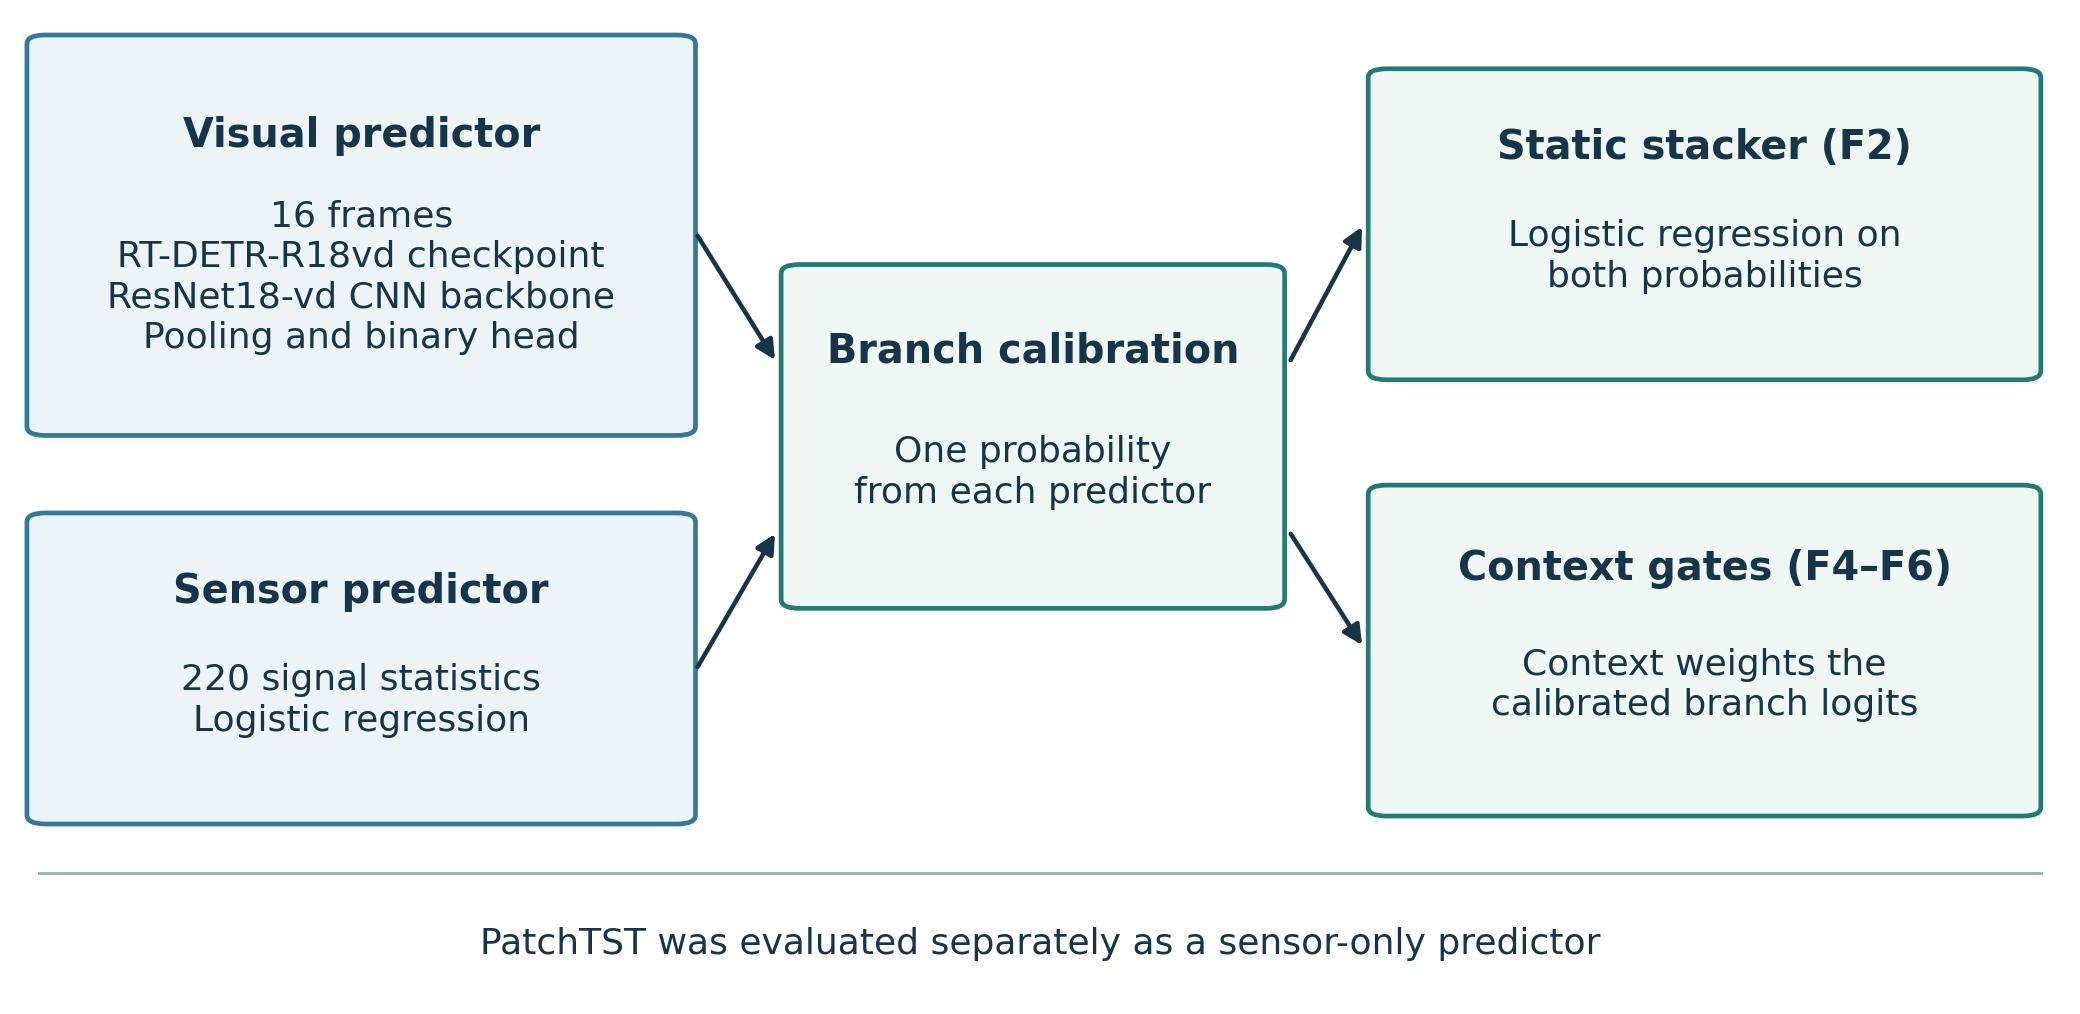
\includegraphics[width=\textwidth]{figures/fusion_interfaces.png}
\displaynote{The stacker and all three gates used the statistical sensor predictor. PatchTST was evaluated separately as a sensor-only comparator in the core experiment. Each branch supplied a calibrated probability. The gates converted those probabilities to logits before weighting them.}
\end{figure}
\section{Component Selection Criteria and Implementation Mapping}
Selection considers target relevance, observation horizon, group support, training exposure, incremental input value, calibration, and computational scope. A frozen representation is attractive when nested fits must remain feasible; a statistical reference is essential when a larger encoder may overfit or be insufficiently trained. An adaptive fusion stage is warranted for investigation when reliability varies and meaningful quality signals exist, but it must still beat an exposure-matched simpler control.

The original visual, audio and sensor question consequently includes implemented and candidate components. AST supplies a pretrained spectrogram-Transformer option, with reported scores distinguishing checkpoint weight averaging from multi-model ensembles and showing task-dependent transfer benefits \citep{P011}. Alignment checks prevented admission of a predictive audio branch here. The published ViT, Video Swin, AST and MOMENT evaluations provide architectural precedents. The executed comparison instead concerns frozen CNN features, statistical sensors, a scratch temporal encoder and explicitly defined fusion interfaces.

The implementation map (Appendix~\ref{app:reproducibility}, \EvidenceRef{E110}{}) records executed paths; Appendix~C lists configuration details. Each performance estimate applies to the combination of components, cohort and metric evaluated in that experiment. The studies did not jointly test all components that performed well individually.
